\chapter{ファイル送信時におけるデータ容量と処理時間の考察} \label{chap:data_time_detail}

始めに、処理速度遅延の原因として以下をあげる。
\begin{itemize}
  \item サーバーの読み書き速度.
  \item サーバーのファイル転送アルゴリズム.
  \item サーバーのファイル転送時におけるパケットサイズ.
  \item サーバー間のネットワーク上の距離.
  \item サーバー間ネットワークの処理性能.
\end{itemize}

KEKとLBNLに設置されているサーバーにおいて、中央データベースへのファイル送信処理時間に差が出る理由について考察する。

ここで、ファイル送信時におけるデータ容量と処理時間の関係は、線形性を示さない。
図\ref{datasize_vs_time_scp}はKEKからLBNLのサーバーにscpコマンドを用いてファイル送信を行い、データ容量と処理時間の関係を取得したものである。
赤線が線形フィットであるが、測定点は優位にずれている。
これはTCP通信においてパケットの送信に輻輳制御\cite{e-1}と呼ばれる技術が使われており、データ送信量を変化させながら情報通信を行っているためである。

\begin{figure}[bpt]\centering
  \begin{center}
    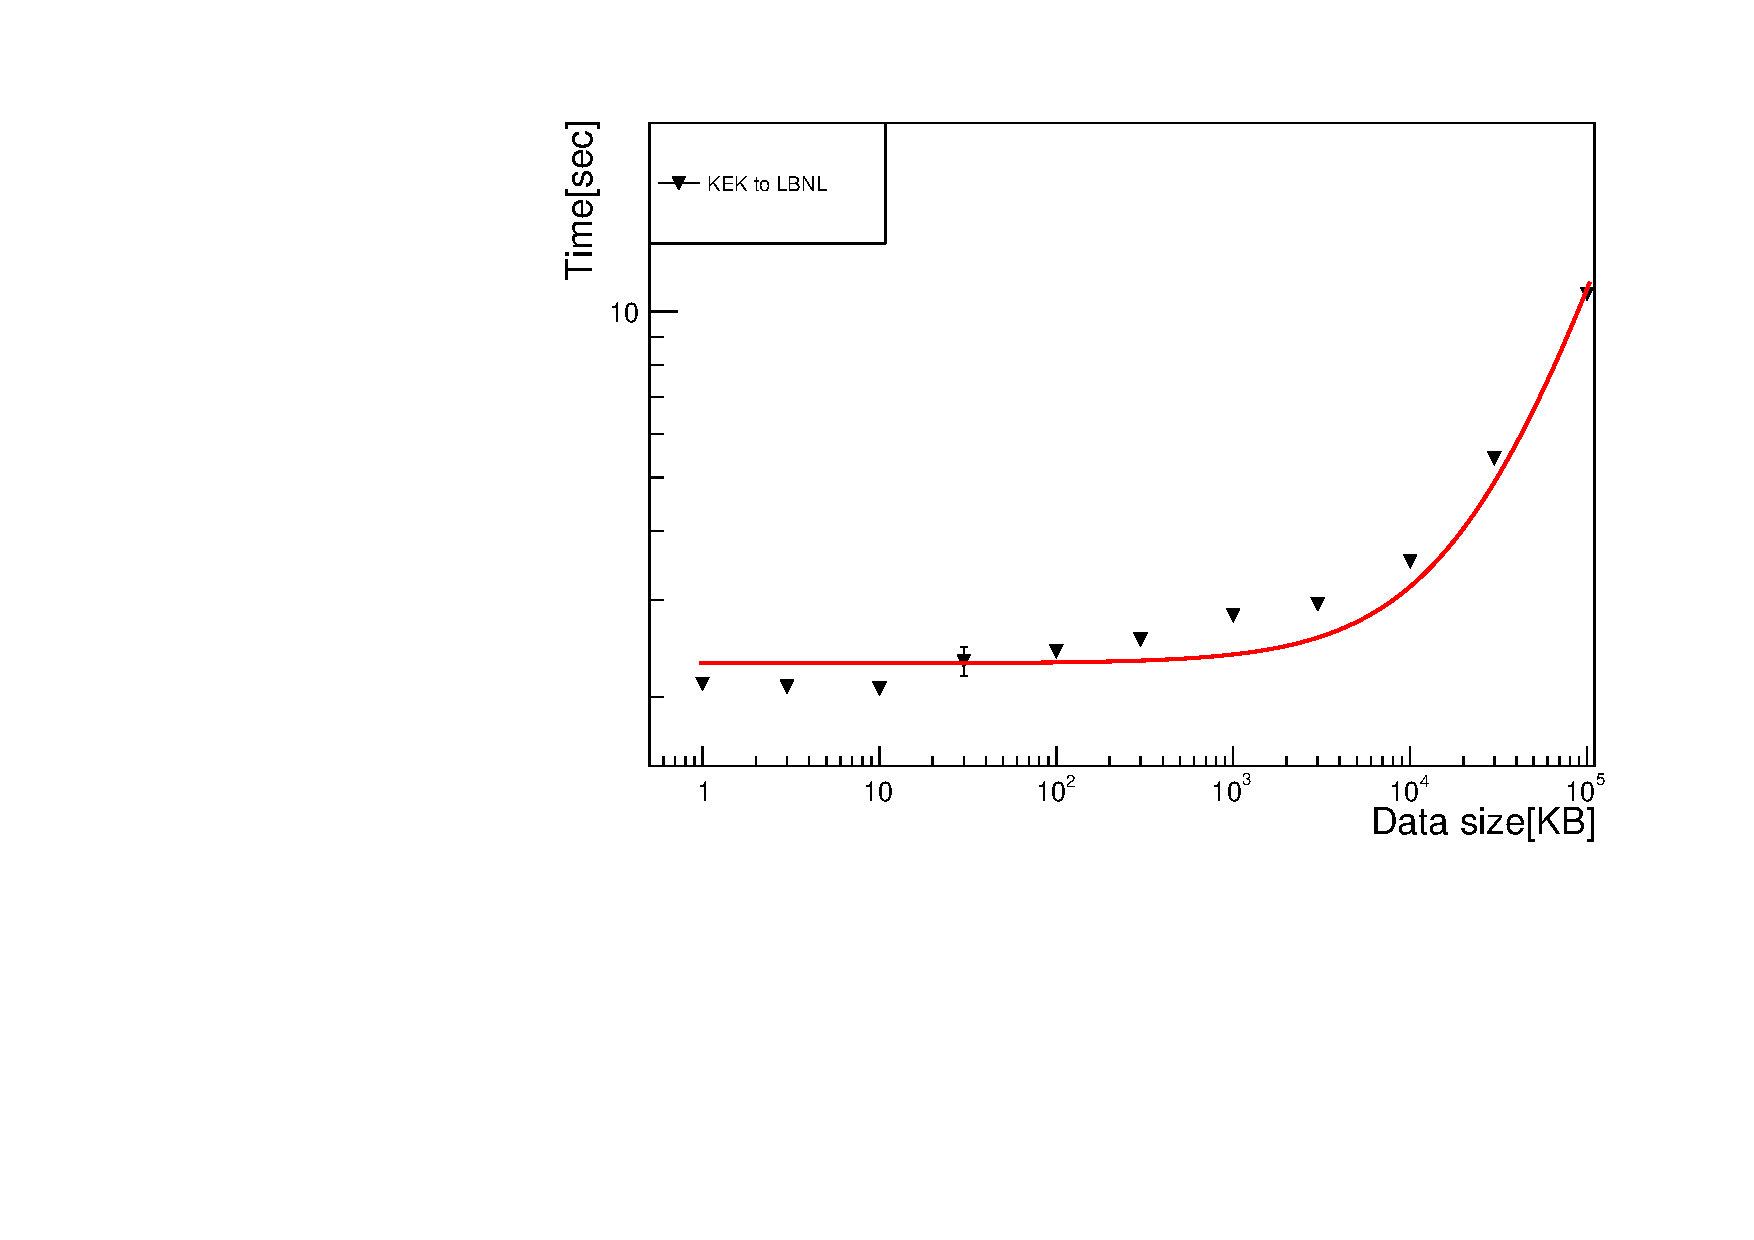
\includegraphics[width=7cm,angle=270]{./datasize_vs_time_scp.pdf}
  \caption[scp送信におけるファイルサイズと処理時間の関係]{scp送信におけるファイルサイズと処理時間の関係。横軸はファイルサイズ、縦軸は時間を示している。赤線は線形フィットを示している。測定点はフィット関数から優位にずれており、scp送信においてファイルサイズと処理時間は線形性を示さないことが分かる。}
  \label{datasize_vs_time_scp}
  \end{center}
\end{figure}

scpによるファイル送信を以下の2つの場合に対して行い、ファイル容量と処理時間の関係を取得した。

\begin{enumerate}
  \item KEKからLBNL.
  \item LBNLからKEK.
\end{enumerate}

結果を図\ref{datasize_vs_time_kek_lbl}に示す。
ここで処理時間に差が生まれる原因について調査したものを以下に示す。
\begin{itemize}
  \item 読み書き速度を測定したところ同程度であった。
  \item 輻輳制御アルゴリズムはCubicをどちらも使用していた。
  \item パケットサイズは変わらなかった。
  \item pingによる応答時間確認は同程度であった(111~msec)。
\end{itemize}

よって各サーバが置かれているローカルネットワークの性能に差があると考えた。
一般的には上りより下りの方が太いと考えると、KEKローカルの上りネットワークの性能が、LBNLローカルの上りネットワークと比べて悪いと考えられる。
これにより、ファイル送信時間に差が生まれている。

\begin{figure}[bpt]\centering
  \begin{center}
    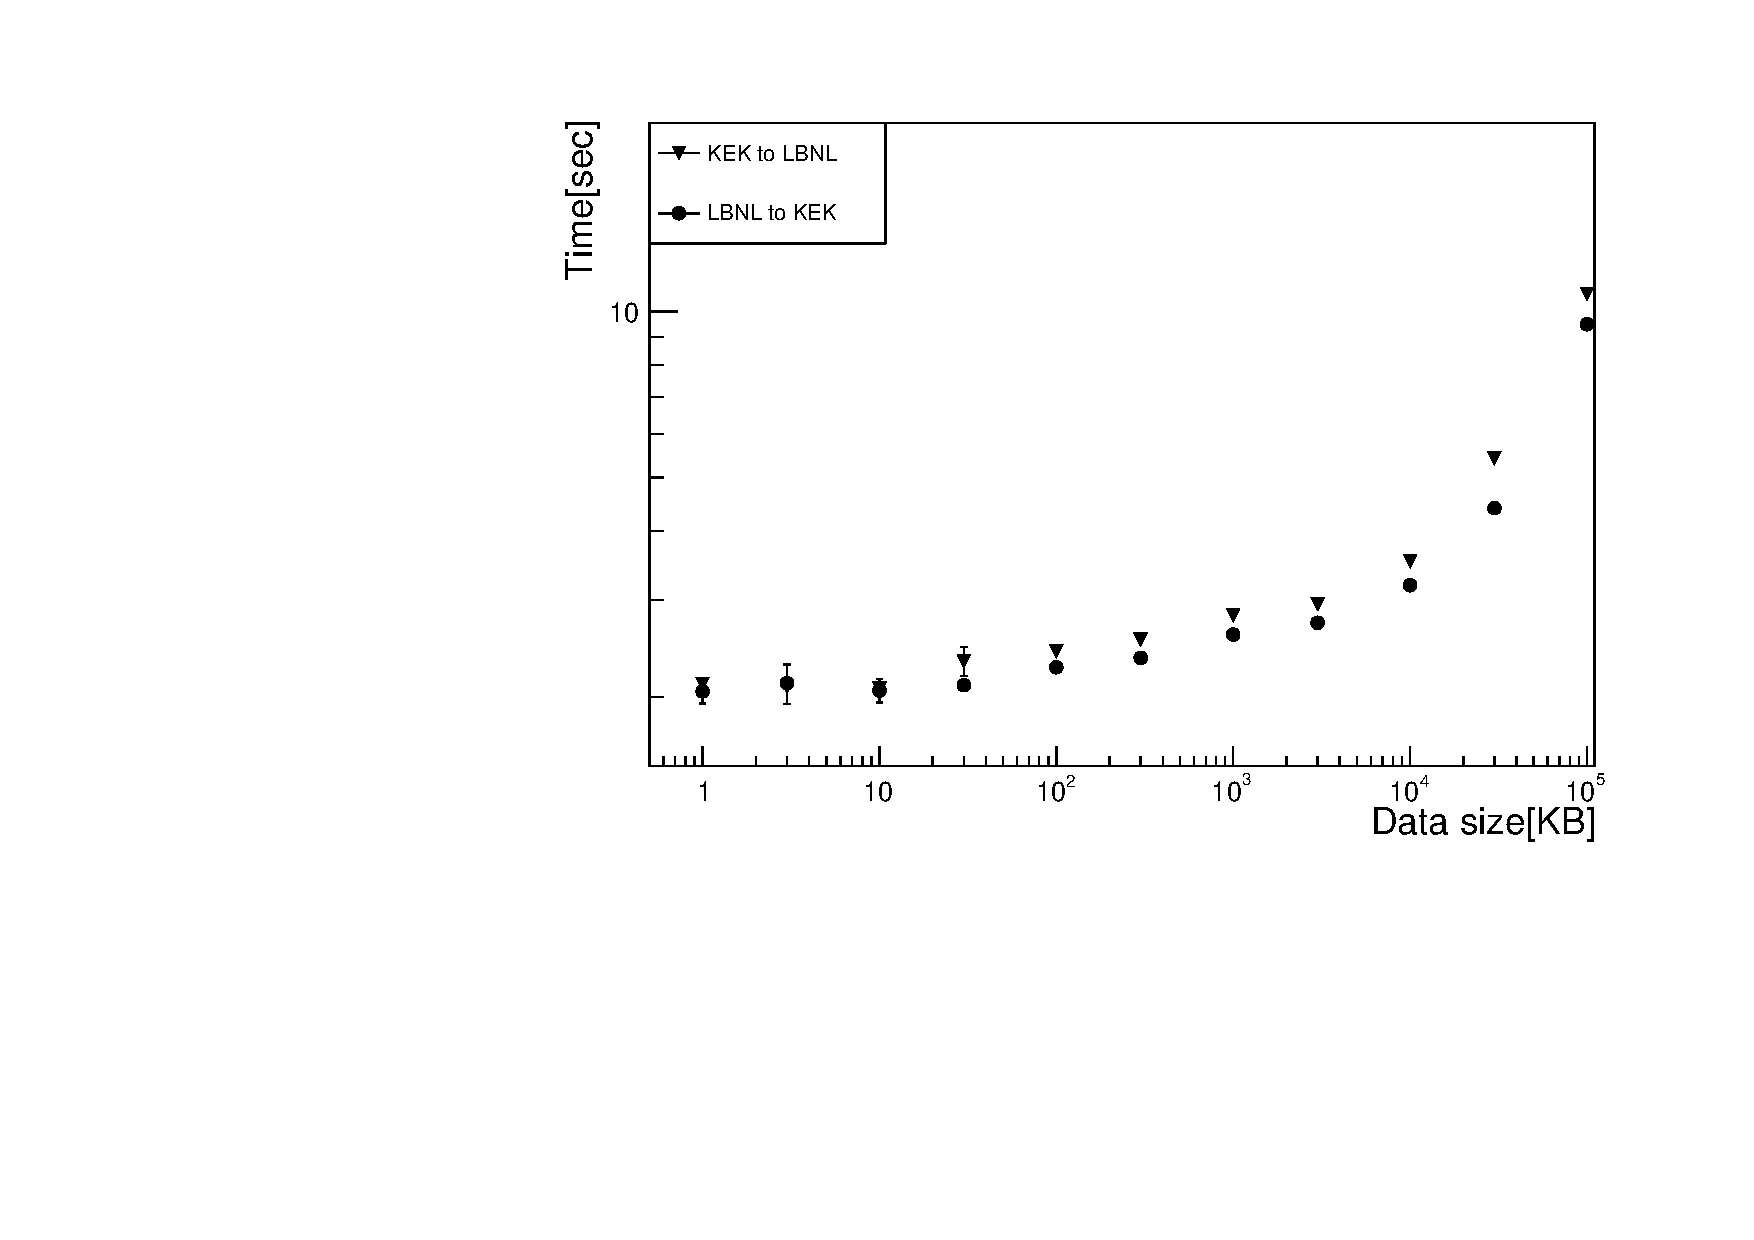
\includegraphics[width=7cm,angle=270]{./scp_kek_lbl.pdf}
  \caption[KEK、LBNL間のファイル送信]{KEK、LBNL間のファイル送信におけるファイルサイズと処理時間の関係。横軸はファイルサイズ、縦軸は時間を示している。三角はKEKからLBNL、丸はLBNLからKEKに送信した場合のものである。比較してKEKからLBNLへのファイル送信の方が時間がかかっている。}
  \label{datasize_vs_time_kek_lbl}
  \end{center}
\end{figure}

次に、下の2つの場合に対して行い、ファイル容量と処理時間の関係を取得した。
\begin{enumerate}
  \item KEKからCERN(Lxplus).
  \item LBNLからCERN(Lxplus).
\end{enumerate}

結果を図\ref{datasize_vs_time_cern}に示す。KEKローカルの上りネットワークは細いため、処理時間に差が生まれる。
加えてこの場合はサーバ間の距離による遅延も含まれていると考えられる。
pingによる応答時間が測定1では170~msec程度なのに対し、測定2は150~msec程度であった。
これも処理速度遅延に影響していると考えられる。

\begin{figure}[bpt]\centering
  \begin{center}
    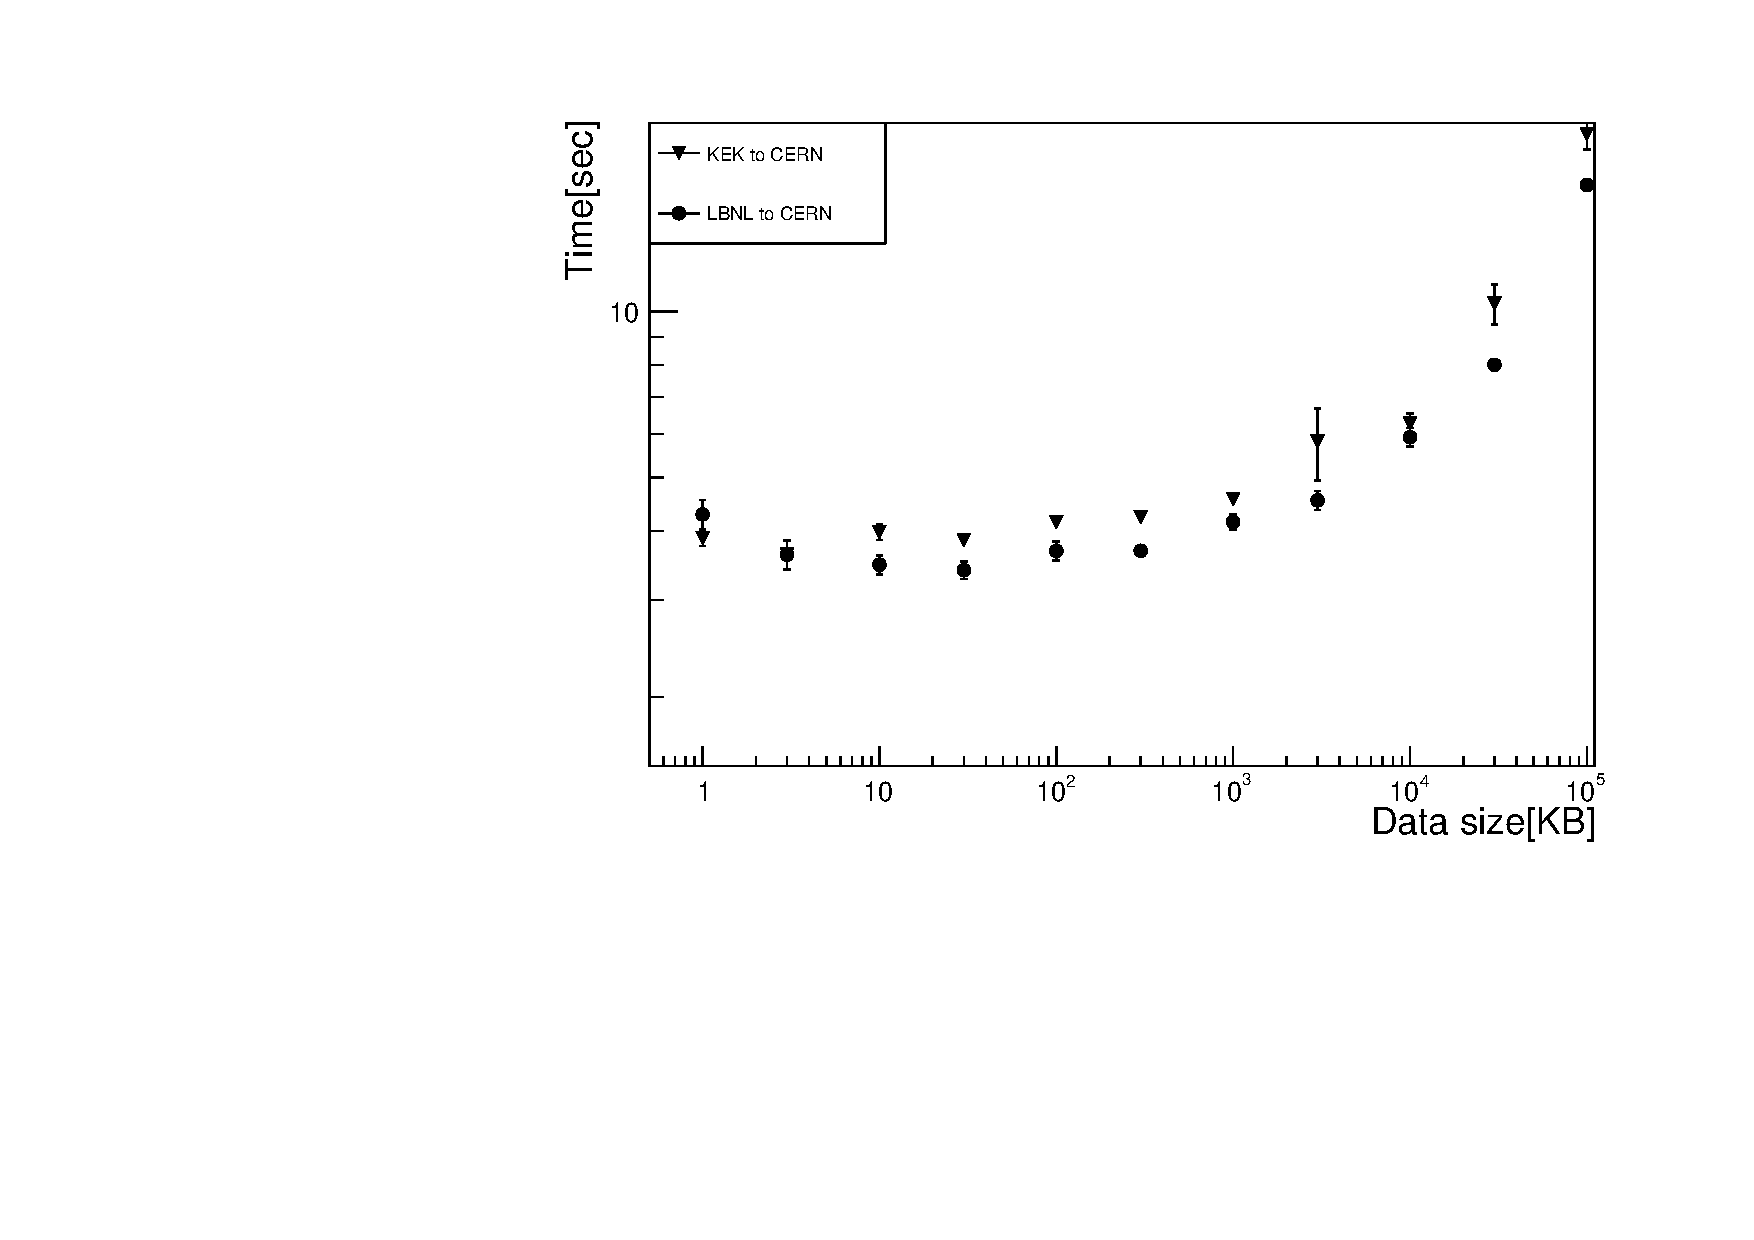
\includegraphics[width=7cm,angle=270]{./scp_to_cern.pdf}
  \caption[KEK、LBNLとCERN間のファイル送信におけるファイルサイズと処理時間の関係]{KEK、LBNLとCERN間のファイル送信におけるファイルサイズと処理時間の関係。横軸はファイルサイズ、縦軸は時間を示している。三角はKEKからCERN、丸はLBNLからCERNに送信した場合のものである。比較してKEKからCERNへのファイル送信の方が時間がかかっている。}
  \label{datasize_vs_time_cern}
  \end{center}
\end{figure}

CERNと中央データベースが地理的に近い距離であることを考慮し、上述したことをまとめるとKEKとLBNLの間で処理時間の差が生まれる要因は以下であると考えた。
\begin{itemize}
  \item ローカルネットワークの性能.
  \item ネットワーク上の距離差.
\end{itemize}

